%By Maria/
 \subsubsection{Pims Login}
Pims User login testes for correct authentication and identification before the user is allowed system access. Further testing was done for user rights and privilages.
\newline

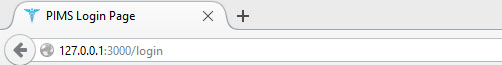
\includegraphics[width=\linewidth]{./Graphics/login.jpg}
\newline

Front end representation
\newline

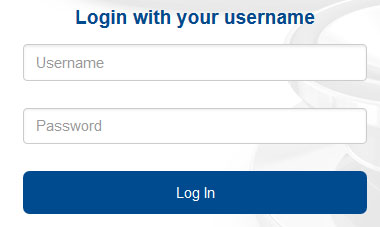
\includegraphics[width=\linewidth]{./Graphics/frontEnd.jpg}
		
User Authentication tested for the following conditions					
	\begin{itemize}
				\item Provide user with access
				\item Retrieve username
				\item Retrieve user password
				\item Fail with empty username and/ or empty password
				\item Return a boolean with regards to user right.
 \end{itemize}
 
 The figure bellow depics the successful testing of the Authentication and checkAdmin functions.
 \newline
 
 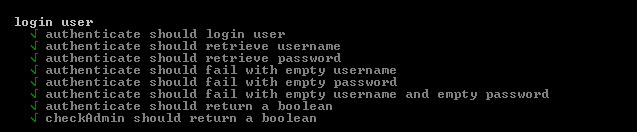
\includegraphics[width=\linewidth]{./Graphics/userResults.jpg}
 
 \subsubsection{Remarks}
 	\begin{itemize}
 				\item Pre-Conditions
 		User does not have access to systme.
 				\item Post-Conditions
 With correct login details, user successfuly gains access into the system with.
 User rights are checked upon login authentication
  \end{itemize}
  
  Both Pre and Post conditions  are considered in the implimentation of the system login. Unit testing successfuly.  tested with no violations to the security of the systm.
 